\documentclass[letterpaper,10pt]{article}

\usepackage{enumitem}
\usepackage{titling}
\usepackage{listings,listings-rust}
\usepackage{url}
\usepackage{soul}
\usepackage{hyperref}
\usepackage{setspace}
\usepackage{subfig}
\usepackage{sectsty}
\usepackage{pdfpages}
\usepackage{colortbl}
\usepackage{multirow}
\usepackage{multicol}
\usepackage{relsize}
\usepackage{amsmath}
\usepackage{wasysym}
\usepackage{fancyvrb}
\usepackage[yyyymmdd]{datetime}
\usepackage{amsmath,amssymb,amsthm,graphicx,xspace}
\usepackage[titlenotnumbered,noend,noline]{algorithm2e}
\usepackage[compact]{titlesec}
\usepackage{XCharter}
\usepackage[T1]{fontenc}
\usepackage[scaled]{beramono}
\usepackage[normalem]{ulem}
\usepackage{booktabs}
\usepackage{tikz}
\usetikzlibrary{arrows.meta,automata,shapes,trees,matrix,chains,scopes,positioning,calc,decorations.pathreplacing}
\tikzstyle{block} = [rectangle, draw, fill=blue!20, 
    text width=2.5em, text centered, rounded corners, minimum height=2em]
\tikzstyle{bw} = [rectangle, draw, fill=blue!20, 
    text width=4em, text centered, rounded corners, minimum height=2em]

\definecolor{namerow}{cmyk}{.40,.40,.40,.40}
\definecolor{namecol}{cmyk}{.40,.40,.40,.40}
\renewcommand{\dateseparator}{-}

\let\LaTeXtitle\title
\renewcommand{\title}[1]{\LaTeXtitle{\textsf{#1}}}

\lstset{basicstyle=\footnotesize\ttfamily,breaklines=true}

\newcommand{\CPP}{C\nolinebreak\hspace{-.05em}\raisebox{.4ex}{\tiny\bf +}\nolinebreak\hspace{-.10em}\raisebox{.4ex}{\tiny\bf +}}
\def\CPP{{C\nolinebreak[4]\hspace{-.05em}\raisebox{.4ex}{\tiny\bf ++}}}

\newcommand{\handout}[5]{
  \noindent
  \begin{center}
  \framebox{
    \vbox{
      \hbox to 5.78in { {\bf ECE459: Programming for Performance } \hfill #2 }
      \vspace{4mm}
      \hbox to 5.78in { {\Large \hfill #4  \hfill} }
      \vspace{2mm}
      \hbox to 5.78in { {\em #3 \hfill \today} }
    }
  }
  \end{center}
  \vspace*{4mm}
}

\newcommand{\lecture}[3]{\handout{#1}{#2}{#3}{Lecture#1}}
\newcommand{\tuple}[1]{\ensuremath{\left\langle #1 \right\rangle}\xspace}

\addtolength{\oddsidemargin}{-1.000in}
\addtolength{\evensidemargin}{-0.500in}
\addtolength{\textwidth}{2.0in}
\addtolength{\topmargin}{-1.000in}
\addtolength{\textheight}{1.75in}
\addtolength{\parskip}{\baselineskip}
\setlength{\parindent}{0in}
\renewcommand{\baselinestretch}{1.5}
\newcommand{\term}{Winter 2020}

\singlespace


\begin{document}

\lecture{24 --- Password Cracking, Bitcoin Mining}{\term}{Patrick Lam \& Jeff Zarnett}

\section*{GPU Application: Password Cracking}

GPUs are good---too good, even---at password cracking. We'll discuss a paper
that proposes a technique to make it harder to crack passwords. This technique
is scrypt, the algorithm behind DogeCoin~\cite{scrypt}. See also \url{http://www.tarsnap.com/scrypt.html}

First, let's talk about acceptable practices for password storage. It is \emph{not}
acceptable engineering practice to store passwords in plaintext. The inevitable security
breach will end with your company sending a ``sorry'' disclosure email to its clients,
and you will be responsible for the ensuing bad publicity. Acceptable practices: {\bf not} plaintext; hashed and salted (we won't discuss salting here but hopefully you remember it from previous courses or other experience.)

\paragraph{Cryptographic hashing.} Instead of storing the plaintext password, you
store a hash of the password, under a cryptographic hash function. One important
property of a cryptographic hash function is that it must be (believed to be a) one-way
function; that is: $x \mapsto f(x)$, the forward direction, must be easy to compute, but
$f(x) \mapsto x$, the inverse mapping, must be hard to compute. Examples of such functions
include SHA-3 and scrypt. 

Some known cryptographic algorithms are already pretty well broken (DES, SHA1) and if you choose one of those then it's like no security at all. Other systems have a broken implementation of the algorithm that is vulnerable to some attack. And even if you chose a good algorithm with no known vulnerabilities in the implementation, you need to choose enough bits (e.g., 512 and not 32), otherwise it's too easy to break...

\paragraph{Not Secret.}
In real life, you can get around the idea of cryptographic hashing by looking on the internet to see if someone's password has already been leaked. Many services are terrible about their password storage policies so if you used the same username and password combination of mycrappywebsite.com and your online banking, then if the mycrappywebsite database gets hacked then the attacker has your user and password already without having to break anything.

\paragraph{First, Check if the Door Is Locked}
As you might imagine, the first thing to try is super common passwords: ``password'', ``system'', et cetera. Users frequently choose common words as passwords and if you just try them all you might get a hit. Choose stronger passwords!

\paragraph{Breaking the hash.} Even if there is no known short computation for the
inverse function, it's always possible to brute-force the password
computation by trying all possible passwords. Think about how GPUs
work. Each potential password is a point in the computation space, and
we compute the hash over all of them simultaneously.  That's a lot of
speedup.

Any website with even slightly decent design will start locking accounts after too many bad login attempts, if not outright banning the caller. But if you get a copy of the database, or at least of some cryptographically-hashed passwords, then a brute force approach is possible.

\paragraph{Arms race: making cracking difficult.} The idea has always been
to make it more difficult to compute the hash function. This does make it longer for the user when they want to log in, but the amount of time to compute a single password is reasonable. However, it's intractable to try all possible passwords, at least with current hardware. 

Even way back,
UNIX passwords forced repeated applications of the hash function to increase the difficulty. The computational power available to us today is of course dramatically more than it was 20 or 30 years ago, and we can reasonably imagine that the computational power in 20 years will vastly exceed what we currently have, making it plausible to crack a password that's effectively uncrackable today. That's okay, just make sure to change your encryption algorithm (and your password!) as needed to stay ahead of the crackers.

Aside: quantum computing won't basically wreck everything we're talking about in virtually zero time. Those are really good for solving problems like asymmetric key encryption (e.g., RSA), but not as good at hashing problems. Fortunately for our banking details.

The main idea behind scrypt is to make hashing expensive in both time and space,
increasing both the number of operations and the cost of brute-forcing. This is how we increase the difficulty to make it implausible to crack in a reasonable amount of time. The only choice that they have to try to break it is, well, to use more circuitry to break passwords (and it will take more time).

Of course, there's always this form of cracking:
\begin{center}
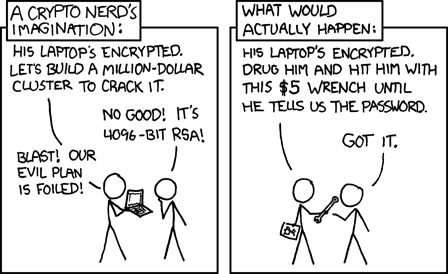
\includegraphics[width=0.5\textwidth]{images/xkcd-538}\\
\hfill (Source: xkcd 538)
\end{center}

\newtheorem{defn}{Definition}

\paragraph{Formalization.} Let's make the notion of ``expensive'' a bit more formal.
The idea is to force the use of the ``most memory possible'' for a given number of
operations. More memory implies more circuitry required to implement.

    \begin{defn}
      A \emph{memory-hard} algorithm on a Random Access Machine is an
      algorithm which uses $S(n)$ space and $T(n)$ operations, where
      $S(n) \in \Omega(T(n)^{1-\varepsilon})$.
    \end{defn}

Memory-hard algorithms are expensive to implement in either hardware or software.

Now, we want to move from particular algorithms to the underlying
functions (that is, we would like to quantify over all possible
algorithms). Intuitively, a \emph{sequential memory-hard function} is
one where (1) the fastest sequential algorithm is memory-hard; and (2)
it is impossible for a parallel algorithm to asymptotically achieve
lower cost.

\paragraph{Existence proof.} Of course anyone can define anything.
It's much better if the thing being defined actually exists. The
scrypt paper then goes on to exhibit ReMix, which is a concrete
example of a sequential memory hard function.

Finally, the paper concludes with an example of a more realistic
(cache-aware) model and a hard function in that context, BlockMix.

\paragraph{Rainbow Tables} So, the brute force approach is the simplest to describe but is computationally intensive, and if a sufficiently-well-designed cryptographic hash function is used it's really tough to actually crack a password. But maybe if we want to crack a password we don't have to always start from zero; maybe we could remember some previous computations so that we could use those answers later. If we calculated the hash of password ``12345'' and we knew what that looked like, if we encountered that hash in the future we could already jump immediately to the answer in our lookup table. This is the basic idea behind \textit{rainbow tables}.

There is a technical paper describing how rainbow tables work, but we'll instead use a much less cryptograhic-expert-level explanation~\cite{rainbowtables}. 

Part of the difficulty with this approach is that it isn't practical, or even really possible, to store the hashes for every possible plaintext (unless the plaintext is very small). So the rainbow table is a compromise between speed and space. The ``reduction'' function maps hashes to plaintext:

\begin{center}
	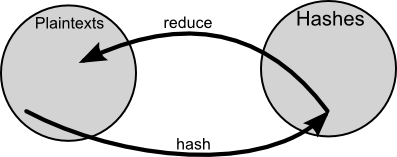
\includegraphics[width=0.4\textwidth]{images/rainbow-tables-reduce.png}\\
	Showing the reduce and hash functions~\cite{rainbowtables}.
\end{center}

This mapping function isn't the inverse of the hash function; it's just some sort of categorization. If the set of passwords to be cracked is, say, six digit numeric, then we compute the hash for a given input (``123456'') and we get some output (``d41d8cd98f00b204e9800998ecf8427e'') which is then reduced (mapped) to some other value (e.g., we'll take the first 6 numbers, 418980). We have another plaintext now, 418980. So we hash this new one, and reduce it, and so on and so on, until some end point ($n$ times, where you choose $n$). 

\begin{center}
	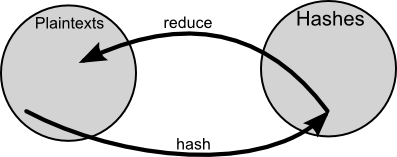
\includegraphics[width=0.4\textwidth]{images/rainbow-tables-reduce.png}\\
	And now we have a chain~\cite{rainbowtables}.
\end{center}

We should do this to develop some number of chains. This is the sort of task you could do with a GPU, because they can do a reduction relatively efficiently. 

Once we have those developed for a specific input set and hash function, they can be re-used forever. You do not even need to make them yourself anymore (if you don't want) because you can download them on the internet... they are not hard to find. They are large, yes, but in the 25 - 900 GB range, which is large  but not ridiculous. I mean, Fallout 76 had a day one patch of 52 GB, and it was a disaster of a game.

Alright, so, you've got them (or made them), but how do we use rainbow tables? Well, for a given hash with an unknown plaintext~\cite{rainbowtables}:
\begin{enumerate}
	\item Look for the hash in the list of final hashes; if there, break out of the loop
	\item If it's not there, reduce the hash into another plaintext and hash the new plaintext
	\item Go back to step 1
	\item If the hash matches a final hash, the chain with the match contains the original hash
	\item Having identified the correct chain, we can start at the beginning of the chain with the starting plaintext and hash, check to see if we are successful (if so, we are done); if not, reduce and try the next plaintext. 
\end{enumerate} 

Like generation, checking the tables for a hit can also be done efficiently by the GPU. Some numbers from \url{http://www.cryptohaze.com/gpurainbowcracker.php.html}: 
\begin{itemize}
	\item Table generation on a GTX295 core for MD5 proceeds at around 430M links/sec.
	\item Cracking a password 'K\#n\&r4Z': real: 1m51.962s, user: 1m4.740s. sys: 0m15.320s
\end{itemize}

Yikes. There is obviously a little bit more complexity to how the rainbow tables work (such as dealing with collisions and loops), but it is clear just how devastatingly effective GPU computations are on breaking passwords.

\section*{The World is Not Enough}
GPUs are great at this, but there are some problems where even the GPU isn't quite the right choice. You have probably guessed it; we're going to talk about Bitcoin. Let's get it out there: I don't think you should mine Bitcoin. This tweet sums up how I would explain Bitcoin to my parents: \url{https://twitter.com/theophite/status/1030225104234373121?lang=en}... and in any case it's pretty uneconomic to mine it and it's terrible for the environment. At the time of writing, the Bitcoin network's carbon footprint is comparable to that of the entire country of Denmark and it uses electricity comparable to the entire power consumption of the country of Austria (source, and for updated figures, see: \url{https://digiconomist.net/bitcoin-energy-consumption}). Alright, enough of that: if you want to know more about why you shouldn't mine Bitcoin, talk to me after class. 

Our guide in this section is~\cite{bitcoin}, a paper that roughly overviews the history of Bitcoin, how it works, and the trend of mining rigs. 

Anyway -- Bitcoin is ``mined'' by doing hash computations, specifically SHA-256. In the beginning, CPUs could be used to mine Bitcoin by performing the calculations. The difficulty of completing the next unit of work increases periodically, so it did not take long for CPU to be inefficient for this purpose. GPUs were the logical step but the quest for more is always ongoing and what do people do when GPU is exhausted?

That's right - they start looking at hardware. Specifically, custom hardware. This works well because the calculations needed are just cryptographic hashing and nothing else. So it's possible to design a system that is optimized to do the few operations in the hash computation (and, xor, rotate, add [modulo], or, right shift) which always happen in a specific order. There's no need for a general purpose CPU or GPU with lots of unnecessary functionality, which just wastes power...

 The first hardware miners were built using FPGAs, but they were quickly replaced by ASIC miners. ASIC miners are much more efficient, both in terms of hashes computed per second but also in terms of power consumption. And the more of these that go online, the harder the computation is and the difficulty of mining Bitcoin (in terms of time) increases. These advances make it basically impossible to mine with the hardware you already have.

So now we've uncovered why you shouldn't mine Bitcoin. If you want to do so in a cost-effective manner (otherwise what's the point), you have to spend money on a mining rig of some sort (which is a significant investment), and pay for the power consumption of it (which is also not zero), and some maintenance is required. And because the difficulty is high and new technology is constantly being released to mine more efficiently, it is quite likely that before long your mining setup costs more to run than is earned in Bitcoin. At which point: don't bother.

This isn't a hardware course so we're not going to invest a lot of time in talking about how one might cleverly design hardware. There are other courses for that, but it's the logical extension of using the GPU, so I thought it might be worth a mention.


\bibliographystyle{alphaurl}
\bibliography{459}


\end{document}
